\chapter{Yushan底层开发手册}

Agent2D是秋山英久博士(日本)开发的一套基于UVA底层的仿真2D底层,汇集了球队底层基本动作和大部分基础问题的解决方案。球队开发伊始,它可以用作参考模板。在后续开发过程中,也可以对其进行编辑、调整。

中国安徽工业大学Yushan队对Agent2D的代码结构和编译方法上进行了优化,形成了编译效率高、可操作性强的底层。IEU队的代码就是基于YushanBase上开始开发的。
\section{框架分析与源码结构}

在Agent2d\_base上进行了结构调整,优化了一系列的makefile。(感谢Yushan\_GF学长)YS的版本rcsc库开放,更利于学习者学习;可执行文件与源码分开,减少赛场失误。

修改过后的类库和球队代码结构如下:
\begin{figure}[htb]
	
\includegraphics{rcsc.png}
	\caption{rcsc库的结构及作用}
\end{figure}


\begin{figure}[H]
	%\usepackage{float}
	
\includegraphics{src.png}
	\caption{src的结构及作用}
\end{figure}

\begin{itemize}
	\item body*.cpp/.h	球员原子动作
	\item bhv*.cpp/.h	组合动作(原子动作特定组合,为实现某种目的),策略,战术
	\item neck*		颈的动作,用于提高信息精度
	\item view*		视角的选用策略
\end{itemize}
\section{开发工具与使用}
欲立其事,必先利其器。在Yushan架构下的2D代码的开发过程中,我们寻找到了一些工具和方法来方便编码和
调试。工具的熟练使用也是我们能够高效工作的基础,希望大家能够熟练的使用下面的工具。
\subsection{代码编辑与编译}
\subsubsection{QT简介}
IDE是×××,

QT是一个跨平台C++图形用户界面应用程序开发框架。它既可以开发GUI程序,也可以开发非GUI程序,比如控制台工具和服务器。QT是面向对象的框架,使用特殊的代码生成扩展以及一些宏,易于扩展,允许组件编程。

QT在编辑上的优势。。。。
\subsubsection{使用QT管理yushan底层}

\subsection{代码调试与分析}

\subsubsection{日志分析}
日志是我们调试代码的一种重要手段,我们之前在命令行下面变成的时候,通常使用输出日志文件的方式来调试代码。
这种可以快速定位程序分支执行情况和错误发生的地方。秋山在Agent2D的开发中,也同样使用了这种方法,并留下了
非常好、非常完善的日志类供开发者使用。
在YushanBase中启动调试功能非常简单,只需修改 data/player_config.conf 下如下参数即可:

秋山教授在soccerwindow2中同样开发了将日志信息可视化的功能,让日志文件可以在soccerwindows中更直观的展示
出来,方便开发者使用,使用方法如下:

当然我们也可以针对自己的程序编写自己的日志记录,比如在调试一个小功能的时候,并不想调用庞大的底层中dlog,
我们可以自己编写文件输入输出代码,来记录调试自己的功能。
\subsubsection{动态调试}
当然日志记录并不能解决所有的问题,比如,在我们在测试中出现了bug,需要复盘曾经出现过的现象,进行动态调整代码
的时候便行不通了。Agent2D在这里也提供了类似蓝鹰DynamicDebug的功能,被称作OfflineMode。
这个功能,通过记录比赛时的全部信息并输出为文件,然后在程序启动调试模式之后,将这些以前记录下的数据“伪装”成服务器发播的信息,供Client程序使用,以实现复盘重现、动态调试的效果。

实际上这种动态调试并不是真正的动态调试,只能一种非实时的程序调试。不过对于我们来说这已经足够了,有了这些东西
我们可以清晰的了解程序的运行情况,尽情的去除bug了!!

offlineMode的启动和使用方法如下:
\subsection{版本控制}

\subsubsection{Git简介} 

Git是一个开源的分布式版本控制/软件配置管理软件。Git可以用于1、管理编程源代码:个人项目、集体项目;2、合作编写文档并用 Git 管理;3、配合 Github/Gitcafe/... 等代码托管网站, 轻松实现代码同步、参与开源项目;等等。Git尤其适合1、个人小项目管理;2、联系紧密的小项目组合作开发;3、多人协作大中型开源项目管理 (如 Github 托管的各类项目)。

Git 的工作流(workflow)设计,以及它对分支(branch)操作的支持十分优秀
Git 由一系列的小工具组成,配合使用完 成工作任务。如: git add, git commit, git reset, git checkout, git remote, git bisect, git diff ......


\subsubsection{Git使用实例}
以 /tmp/tmp 目录作为项目的工作目录, 在其中创建一个 README 纯文本文件, 并使用 Git。

第一步:初始化 Git 版本库
1. 进入工作目录(如,使用cd),并输入
\begin{Code}
	git init
	初始化空的 Git 版本库于 /home/wt/.git/
\end{Code}
2. 初始化配置 :
\begin{Code}
	git config --global user.name "Wu Tong"
	git config --global user.email "1159559828@qq.com"
\end{Code}
查看当前工作树状态:
\begin{Code}
	git status
	位于分支 master
	无文件要提交,干净的工作区
	随时运行 git status 即可查看当前状态, 工作情况尽在掌握之中。
\end{Code}

第二步:编辑文件
3. 创建一个新文件并写入内容:
\begin{Code}
	touch README
	echo "Hello World!" > ./README
	查看文件内容:
	cat ./README
\end{Code}

第三步:添加到暂存区

4. 添加 README 文件至暂存区:
\begin{Code}
	git add ./ README
\end{Code}


5. 进行初始提交:
\begin{Code}
	git commit -m 'First Commit'
\end{Code}




\section{开发心得}

\subsection{学习优秀代码}
作为一个2D的初学者,最初一般都是从学习别人的代码开始的。2D项目发展到现在,我们已经有很多优秀的代码可以学习。比如Helios08年的代码,2011年国内各个球队公开的代码,以及各个公布底层的代码。其中都包含大量的优秀代码值得大家学习。

但是对于一个如此庞大的项目学起来自然是很费力的,所以一定的方法是有必要的。在2年多的时间里,我们2014届的队员大部分的时间都在学习别人的代码,也总结了一些学习的方法,希望对大家有帮助。

\subsubsection{框架学习}
在学习之前,我们必须要对自己要学习的东西有一定的了解,也就是说如果我们想深入的学习这些东西,我们到底要从哪里下手,这就是需要了解清楚整体程序的框架。这里以YushanBase为例,进行讲解。

上一节中我们已经了解了基本的代码的结构和功能,如此繁多的模块是如何组织在一起的。任何一个程序都会从main()开始,我们的机器人程序也不例外。程序运行的流程图如下。
	\begin{figure}[H]
		\centering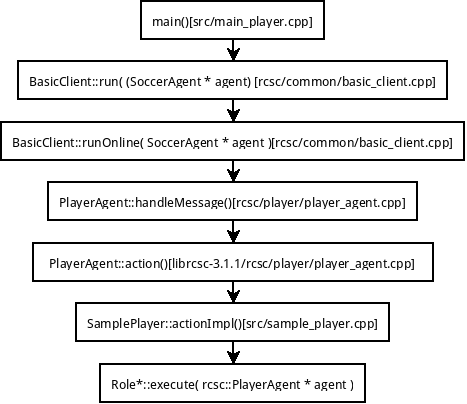
\includegraphics[width=0.65\textwidth]{run.png}	
		\caption{ agent 流程图}
	\end{figure}


毋庸置疑,任何代码的执行都是从main函数开始的,agent也不例外。
每个agent的main函数首先设置和判断一下signal,然后转入BasicClient
类的run ()方法启动agent。接着进入BasicClient的runOnline ()方法启动在
线Agent, runOnline () 方法调用PlayerAgent类的handleMessage ()方法
处理获得的信息,处理完之后handleMessage () 方法调用在同一个类中
的方法action()进行动作决策。在action()方法依次进行actionImpl() (body
动作决策) ,doArmAction() (手臂动作决策),doViewAction() (视觉决策),
doNeckAction() (颈部动作决策)以及communicationImpl () (通信决策) 。
这里要注意一下, PlayerAgent类的actionImpl() 是一个纯虚函数,也就是说
实际的动作决策是在其子类SamplePlayer的方法actionImpl()中完成的。这就是整个Yushan架构运行的流程,每个周期都会往复运转。

PlayerAgent类的actionImpl() 是一个纯虚函数,所以我们从它的子类SamplePlayer的方法actionImpl() 开始看起。方法actionImpl() 首先根据该agent的球员号码创建该agent对应的球员角色,然后当比赛模式为playon的时候调用该类球员角色的execute () 方法进行该类球员角色的body动作决策。当然, actionImpl() 还进行了许多非playon模式下的agent决策。

球员角色的基类是SoccerRole,派生了8个子类RoleCenterBack,RoleCenterForward,RoleDefensiveHalf……(在src的8个以role开头的头文件中定义),分别对应于场上的前锋,中场,后卫等等。球队策略中是根据agent的号码生成该agent对应的球员角色。在现实的比赛中,这些球员角色的区别是很明显的(比如说前锋活跃在中前场,经常射门,后卫活跃在后场,经常大脚解围等),那么在代码中,这些区别是如何实现的呢?这些区别agnet2D的底层为我们实现了一些,但是大部分还是靠我们自己编写代码来实现,也就涉及到各种模型的建立。

上面说到了,agent的body动作决策实际上交给了该类agent对应的球员角色,那么我们现在来看看每类角色到底是如何进行决策的。在agent2D的底层源代码中,八类角色的决策代码几乎是一模一样的(守门员除外),都是先判断自己是否是持球队员,如果是,则按照bhv_basic_offensive_kick.cpp文件中的hv_BasicOffensiveKick::execute()方法进行决策,如果不是,则按照bhv_basic_move.cpp文件中的hv_BasicMove::execute()方法进行跑位或者截球等决策。这一部分就是我们工作的重心,我们要修改这8个文件,使球队能够按照我们的决策来进行比赛。这里大家重点注意一下,agent2d底层已经为搭建了一个决策框架:作者将整个球场划分为10个区域,每类角色的球员可以在这10个区域中进行单独决策,以适应我们的决策需要。
\subsubsection{模型学习}
所谓模型,就是球赛中一些战术或动作的处理方法(包括理论和代码)。通常一个队伍会建立一个模型库\footnote{参考第五章},以收集需要开发的功能和基本思路,以使球队有完整的技术路线。所以真正的技术一般都会体现在这一部分,也就是说这里才是比赛中真正较量的地方。作为一个初学者,我们一般都先学习其他人的模型开始的。

这里以一个简单的学习Helios2008边后卫和中后卫的防守运动为例子,讲解如何学习前人的模型。首先比较一下下面两个代码\footnote{由于篇幅限制已去掉注释,copyright by Helios} 。

\begin{Codex}[label=bhv_side_back_defensive_move.cpp]
bool
Bhv_SideBackDefensiveMove::execute( PlayerAgent * agent )
{
	dlog.addText( Logger::ROLE,
	__FILE__": Bhv_SideBackDefensiveMove" );

	if ( Bhv_BasicTackle( 0.85, 50.0 ).execute( agent ) )
	{
		agent->debugClient().addMessage( "SB:Def:Tackle" );
		return true;
	}
	
	if ( doIntercept( agent ) )
	{
		return true;
	}
	
	if ( doAttackBallOwner( agent ) )
	{
		dlog.addText( Logger::ROLE,
		__FILE__": attack to ball owner" );
		return true;
	}
	
	if ( doEmergencyMove( agent ) )
	{
		return true;
	}
	
	doNormalMove( agent );
	return true;
	
}
\end{Codex}

\begin{Codex}[label=bhv_center_back_defensive_move.cpp]
bool
Bhv_CenterBackDefensiveMove::execute( PlayerAgent * agent )
{
	dlog.addText( Logger::TEAM,
	__FILE__": Bhv_CenterBackDefensiveMove" );
	
	if ( Bhv_BasicTackle( 0.85, 50.0 ).execute( agent ) )
	{
		agent->debugClient().addMessage( "CB:Def:Tackle" );
		return true;
	}
	
	if ( doIntercept( agent ) )
	{
		return true;
	}
	
	if ( doGetBall( agent ) )
	{
		return true;
	}
	
	doNormalMove( agent );
	return true;
	
}
\end{Codex}

比较这两个代码我们可以看到不同角色的球员策略大不相同。边后卫采取的是比较激进的策略,进行攻击对手和紧急补位;而中后卫采取的是getball的策略形成压制势力,防止对方突破。这里就可以看出一个模型只有用在一个正确的位置才能发挥其作用。这里面提到的几种防守的解决方案都是防守中可取的一些方法,下面对其攻击持球者的模型进行分析。

\begin{Codex}[label=bhv_side_back_defensive_move.cpp]
bool
Bhv_SideBackDefensiveMove::doAttackBallOwner( rcsc::PlayerAgent * agent )
{
	const rcsc::WorldModel & wm = agent->world();
	
	const int mate_min = wm.interceptTable()->teammateReachCycle();
	const int opp_min = wm.interceptTable()->opponentReachCycle();
	
	const AbstractPlayerObject * fastest_opp = wm.interceptTable()
						->fastestOpponent();
	
	if ( mate_min < opp_min )
	{
		dlog.addText( Logger::ROLE,
		__FILE__": doAttackBallOwner() ball owner is teammate" );
		return false;
	}
	
	if ( ! fastest_opp )
	{
		dlog.addText( Logger::ROLE,
		__FILE__": doAttackBallOwner() no opponent" );
		return false;
	}
	
	const Vector2D opp_trap_pos = wm.ball().inertiaPoint( opp_min );
	
	const Vector2D home_pos = Strategy::i().getPosition( wm.self().unum() );
	const PositionType position_type = Strategy::i().
			getPositionType( wm.self().unum() );
	
	const MarkTable & mark_table = Strategy::i().markTable();
	const AbstractPlayerObject * mark_target = 
				mark_table.getTargetOf( wm.self().unum() );
	const AbstractPlayerObject * free_attacker = 
			static_cast< AbstractPlayerObject * >( 0 );
	
	if ( mark_target )
	{
		dlog.addText( Logger::ROLE,
		__FILE__": doAttackBallOwner() mark_target= %d (%.1f %.1f)",
		mark_target->unum(),
		mark_target->pos().x, mark_target->pos().y );
		
		//
		// find other free attacker
		//
		const AbstractPlayerCont::const_iterator o_end = wm.allOpponents().end();
		for ( AbstractPlayerCont::const_iterator o = wm.allOpponents().begin();
		o != o_end;
		++o )
		{
			const AbstractPlayerObject * marker = mark_table.getMarkerOf( *o );
			if ( marker ) continue; // exist other marker
			if ( (*o)->pos().x > mark_target->pos().x + 10.0 ) 
				continue; // no attacker
			if ( ( position_type == Position_Left
			&& (*o)->pos().y < mark_target->pos().y + 10.0 )
			|| ( position_type == Position_Right
			&& (*o)->pos().y > mark_target->pos().y - 10.0 )
			|| ( position_type == Position_Center
			&& std::fabs( (*o)->pos().y - mark_target->pos().y ) < 10.0 )
			)
			{
				free_attacker = *o;
				break;
			}
		}
	}
	
	if ( free_attacker )
	{
		dlog.addText( Logger::ROLE,
		__FILE__": doAttackBallOwner() exist free_ataccker= %d (%.1f %.1f)",
		free_attacker->unum(),
		free_attacker->pos().x, free_attacker->pos().y );
	}

	const double min_y = ( position_type == Position_Right
	? 2.0
	: -31.5 );
	const double max_y = ( position_type == Position_Left
	? -2.0
	: +31.5 );
	
	if ( fastest_opp == mark_target )
	{
		dlog.addText( Logger::ROLE,
		__FILE__": doAttackBallOwner() fastest_opp == mark_target, %d (%.1f %.1f) trap_pos=(%.1f %.1f)",
		mark_target->unum(),
		mark_target->pos().x, mark_target->pos().y,
		opp_trap_pos.x, opp_trap_pos.y );
		Rect2D bounding_rect( Vector2D( -50.0, min_y ),
		Vector2D( -5.0, max_y ) );
		if ( Bhv_GetBall( bounding_rect ).execute( agent ) )
		{
			agent->debugClient().addMessage( "SB:Def:GetBall(1)" );
			return true;
		}
	}

	if ( ! mark_target )
	{
		dlog.addText( Logger::ROLE,
		__FILE__": doAttackBallOwner() no mark target.
		 ball_owner=%d (%.1f %.1f) trap_pos=(%.1f %.1f)",
		fastest_opp->unum(),
		fastest_opp->pos().x, fastest_opp->pos().y,
		opp_trap_pos.x, opp_trap_pos.y );
		
		if ( opp_trap_pos.x < home_pos.x + 10.0
		&& ( std::fabs( opp_trap_pos.y - home_pos.y ) < 10.0
		|| ( position_type == Position_Left
		&& opp_trap_pos.y < home_pos.y )
		|| ( position_type == Position_Right
		&& opp_trap_pos.y > home_pos.y ) )
		)
		{
			dlog.addText( Logger::ROLE,
			__FILE__": doAttackBallOwner() no mark target. attack " );
			Rect2D bounding_rect( Vector2D( -50.0, min_y ),
			Vector2D( -5.0, max_y ) );
			if ( Bhv_GetBall( bounding_rect ).execute( agent ) )
			{
				agent->debugClient().addMessage( "SB:Def:GetBall(2)" );
				return true;
			}
		}
	}
	
	return false;
}
\end{Codex}
这个代码的条例非常清晰,首先进行盯人对象的选择,然后对盯人对象的分析,如果球员是最快的球员,就要去getball;同样是使用getball,边后卫的getball就目的性更明确,成功率增高了。
\subsection{优秀编码习惯}

条件编译

模块思想

版本控制


\section{常用的底层模型类}
\subsection{worldmodel}

\subsubsection{世界模型}
Librcsc 库中提供了 WorldModel 类,用来管理球员智能体的内部模型。 WorldModel类 Protected继承PlayerAgent 类的成员。如果 PlayerAgent 或它的派生类要获取运动场的信息,那就必须从 WorldModel 中获取。 WorldModel 类的成员中, SelfObject 类管理球员本身, BallObject 类用于管理球员和球信息,PlayerObject 类信息的容器也是其成员。其他的,包括当前时间、估计越位线也是他的成员,比如 InterceptTable 类来存储球的所有者判断信息。
\subsubsection{WorldModel访问}

%\begin{table}[htbp]
	\begin{tabular}{p{0.9\columnwidth}}
		\hline
		const GameTime \& getTime() const \\ 返回当前的仿真周期。\\
		\hline
		const GameMode \& getGameMode() const\\
		返回了比赛的当前运行模式的信息。\\
		\hline
		SideID getOurSide() const\\
		返回你的球队属于右或左侧信息。\\
		\hline
		const SelfObject \& self() const\\
		PlayerAgent本身的信息。\\
		\hline
		const BallObject \& ball() const\\
		球的信息\\
		\hline
		const PlayerCont \& teammates() const\\
		已明确球衣号码的队友\\
		\hline
		const PlayerCont \& unknownTeammates() const\\
		球衣号码不明的队友\\
		\hline
		const PlayerCont \& opponents() const\\
		已明确球衣号码的对方球员。\\
		\hline
		const PlayerCont \& unknownOpponents() const\\
		未知球衣号码的对方球员 \\
		\hline
	\end{tabular}
%\end{table}

%\begin{table}[htbp]
\begin{tabular}{p{0.9\columnwidth}}
	\hline
		const PlayerCont \& unknownPlayers() const\\
		身份无法识别球员。 \\
	\hline
		const PlayerPtrCont \& getTeammatesFromSelf() const\\
	将我方球员按照与自身距离由近及远排序。\\ 
	\hline
		const PlayerPtrCont \& getOpponentsFromSelf() const\\
		将对方球员按照与自身距离由近及远排序,也包含不能被识别的球员。\\
	\hline
		const PlayerPtrCont \& getTeammatesFromBall() const\\
		将我方球员按照与球d的距离由近及远排序。\\
	\hline
		const PlayerPtrCont \& getOpponentsFromBall() const\\
		将对方球员按照与球的距离由近及远排序,也包含不能被识别的球员。 \\
	\hline
		const PlayerObject * getOpponentGoalie() const\\
		返回对方守门员的指针。如果它不存在,则返回NULL。 \\
	\hline
		const PlayerObject * getTeammateNearestTo( const Vector2D \& point, const int count thr, double * dist to point ) const\\
		置信度count_thr下,返回距离point点最近的我方球员指针。若没有满足该条件的球员,则返回NULL。若dist_to_point不为NULL,则该球员到point之间的距离将会被保存(到dist_to_point中?) \\
	\hline
		const PlayerObject * getOpponentNearestTo( const Vector2D \& point,const int count thr, double * dist to point ) const\\
		类似上条,只是 对方球员版getTeammateNearestTo()。\\
	\hline
		const PlayerObject * getTeammate( const int unum ) const\\
		返回球衣号码为unum的我方球员指针,如果不存在,则返回NULL\\
	\hline
		const PlayerObject * getOpponent( const int unum ) const 
		类似上条,只是 对方球员版getTeammate()。\\
	\hline
		bool existKickableTeammate() const\\
		如果认定可能踢到球的我方球员为村内状态,返回true。 \\
	\hline
		bool existKickableOpponent() const\\
		对方球员版本existKickableTeammate() \\
	\hline
		const InterceptTable * getInterceptTable() const\\
		返回一个指向InterceptTable实体的const指针。 \\
	\hline
		int getDirCount( const AngleDeg \& angle ) const\\
		向angle方向观测最后一个周期。可作为场地区域的可信赖信息使用。(返回的整数究竟做什么用,没明白) \\
	\hline
		HeteroID getTeammateHeteroID( const int unum ) const\\
		返回球衣号码为unum的我方球员类型ID \\
	\hline

\end{tabular}
%\end{table}

\begin{tabular}{p{0.9\columnwidth}}
	\hline	
		const double \& getOffsideLineX() const\\
		估计越位线的横坐标值。\\
	\hline	
\end{tabular}	

\subsection{SelfObject}
\begin{tabular}{p{0.9\columnwidth}}
	\hline
		int unum() const; \\
		球衣号码\\
	\hline
		bool goalie() const; \\
		判断是否为守门员\\
	\hline
		const PlayerType \& playerType() const; \\
		异构球员的参数\\
	\hline
		cons Vector2D \& pos() const; \\
		位置坐标.\\
	\hline
		const Vector2D \& vel() const; \\
		速度.\\
	\hline
		const AngleDeg \& body() const; \\
		身体的绝对方向\\
	\hline
		const AngleDeg \& neck() const; \\
		头与身体朝向的相对角度\\
	\hline
		const AngleDeg \& face() const; \\
		头的绝对方向.\\
	\hline
		const ViewWidth \& viewWidth() const; \\
		当前的视角的大小\\
	\hline
		const GameTime \& catchTime() const; \\
		最后接/持球的时间\\
	\hline
		const double \& stamina() const; \\
		体能值\\
	\hline
		const double \& effort() const; dash \\
		与 Dash 命令效果相关联的体能值。\\
	\hline
		bool isKickable() const;\\
		能否踢到球。\\
	\hline
		const double \& kickRate() const kick \\
		实现 kick 命令的成效比例。它是由playerType() 的参数以及与球的位置关系来确定。\\
	\hline 


\end{tabular}

\begin{tabular}{p{0.9\columnwidth}}
	\hline	
		const double \& dashRate() const dash \\
		实现 dash 命令的成效比例。由playerType() 和 effort() 工作的参数来确定。 \\
	\hline
		const double \& tackleProbability() \\
		当前推算的成功概率。取[0,1]之间的实数值\\
	\hline	
\end{tabular}

\subsection{BallObject}
\begin{tabular}{p{0.9\columnwidth}}
	\hline
const Vector2D \& pos() const\\
位置坐标。 \\
\hline
int posCount() const\\
最后一个周期观测到的位置,作为可靠位置信息。 \\
\hline
const Vector2D \& rpos() const\\
从 SelfObject 出发的相对位置坐标。 \\
\hline
const Vector2D \& vel() const\\
速度。 \\
\hline
int velCount() const\\
最后一个周期观测到的速度,作为可靠速度信息使用。 \\
\hline
const double \& distFromSelf() const\\
与 SelfObject 之间的距离。 \\
\hline
const double \& distFromSelf() const\\
与 SelfObject 之间的绝对方向。 \\
\hline
Vector2D inertiaTravel( int cycle ) const\\
如果没有附加的加速度时,周期内的总移动向量\\
\hline
Vector2D inertiaPoint( int cycle ) const\\
如果没有附加的加速度时,循环后的位置。 \\
\hline
Vector2D inertiaFinalTravel() const\\
如果没有附加的加速度时,直到速度为0之前的总移动向量\\
\hline
Vector2D inertiaFinalPoint() const\\
如果没有附加的加速度时,速度变为0时的位置坐标。\\
\hline
\end{tabular}

\subsection{PlayerObject}
\subsubsection{PlayerAgent的访问}

Playeragent类包含WorldModel类和 ActionEffector类的成员变量。如果想从SampleAgent访问这些的话,可以使用如下成员函数。
\subsubsection{PlayerAgent成员}

\begin{tabular}{p{0.9\columnwidth}}
	\hline	
const WorldModel \& world() const;\\
返回一个WorldModel类实体的const引用/常量参照?。\\ 
	\hline
const ActionEffector \& effector() const;\\
返回一个ActionEffector类实体的const引用/常量参照?。\\
	\hline	
\end{tabular}



\subsubsection{PlayerObject 容器}

WorldModel存有PlayerObject作为其成员变量。对于观察到的多个球员(信息),将被存储在PlayerObject STL的容器中进行管理。

为了减少类型的量,PlayerObject容器通过typedef定义下列两种类型。

\begin{Code}
typedef std::list< PlayerObject > PlayerCont
typedef std::vector< PlayerObject * > PlayerPtrCont
\end{Code}

PlayerCont将用于存储PlayerObject的实例。对于需要频繁增删元素的情况,可使用std::list作为容器。

PlayerPtrCont用于保存PlayerObject的指针。该指针指向存储在PlayeCont的实例。为了实现快速调用,可使用的std :: vector。每当球员智能体的内部状态被更新时,即每当PlayerCont的内容要发生变化的时候, PlayerPtrCont就要进行重新调整。请注意,被存储的值是一个指针。


\subsection{InterceptTable}
InterceptTable类,从worldmodel内保留的信息预测出每名球员捕捉到球所必需的周期数,并将这一结果保存。在球员智能体决策时,可以参照捕捉到球的周期数,从而来判断哪只队伍的哪位球员正在持球。

\subsubsection{WorldModel 成员函数}
\begin{tabular}{p{0.9\columnwidth}}
	\hline	
int getSelfReachCycle() const\\
预测selfobject(球员智能体本身)捕获球的的周期数。\\ 
	\hline	
int getTeammateReachCycle() const\\
预测我方球员捕获球的周期数的最小值。 \\
	\hline	
int getOpponentReachCycle() const\\
预测对方球员捕获球的周期数的最小值。 \\
	\hline	
const PlayerObject * getFastestTeammate() const\\
预测最早捕获球的队友球员的指针*\\
	\hline	
const PlayerObject * getFastestOpponent() const\\
预测最早捕获球的对方球员的指针*\\
	\hline	
\end{tabular}



\subsection{ActionEffector}
相较于WorldModel,ActionEffector是用来记录球员智能体已执行或将要实施的动作,并推测其效果。例如,如果想要一边改变身体朝向,一边将头转向某一位置,那么,你必须掌握身体最终的朝向然后再转头才比较可行。这些可能尚未在rcssserver中得到体现,但是还是由ActionEffector来负责管理已经执行和将要实施的动作。

PlayerAgent类包含有一个ActionEffector类的成员变量。如果需要参考球员决策时使用的信息,就可以使用下面的成员函数。

\subsubsection{ActionEffector成员 }
\begin{tabular}{p{0.9\columnwidth}}
	\hline	
AngleDeg queuedNextMyBody()const; \\
在下一个周期中的身体方向。 \\
	\hline	
的Vector2D queuedNextMyPos()const; \\
下一个周期的位置坐标。 \\
	\hline	
的Vector2D queuedNextBallPos()const;\\ 
在下一周期中球的位置。 \\
	\hline	
的Vector2D queuedNextBallVel()const;\\ 
下一周期球的速度。 \\
	\hline	
AngleDeg queuedNextAngleFromBody(const Vector2D \& target) const; \\
从在下一周期中的目标位置与身体相对方向。 \\
	\hline	
ViewWidth queuedNextViewWidth()const; \\
下一个周期的视角。\\
	\hline	
\end{tabular}


\section{球队开发中的常用方法和模型}
底层的原子动作


%dointention	意图;\\
%doforcekick\\
%doshoot		射门(优先级最高);\\
%doprocess\\
%dopreprocess	如果被冻结(铲球失败等)只看(转脖子);开场前,进球后,位置如果不对,找位置;球员信息不准,观察(维护信息);\\
%非play_on模式:	free_kick 自由球; goal_kick 门球; indirect_free_kik 直接任意球; kick_in 角球; kick_off 开球;\\
%target_point, dist_thr, dash_power\\

\subsection{底层中的原子动作}
底层中存在一些原子动作,可以在server中直接注册动作的命令。
最常见的如下:doKick(),doDash(),doTurn(),doCatch(), doMove(),doTackle(),doTumNeck(),doChangeView(), doPointTo()等动作,这些方法属于PlayerAgent类,均可以使用agent->doKick()方法使用。其实以上的一系列动作在内部均使用ActionEffector类中的set系列方法来将每个动作及其参数转换为发送给server的命令。

以下以doKick为例说明其调用过程。

首先使用 Agent->doKick( power,dir),调用 PlayerAgent 中的 doKick 命令,此处的 power 和dir需要自己计算。
然后在doKick方法中对一些限制条件进行判断,如是否可踢,是否正在铲球状态等,
然后通过ActionEffector进行动作的设定,在ActionEffector中使用setICick(power,dir)方法, 该方法将参数进行规格化,转换成可直接发送给server的参数,最后通过 PlayerBodyCommand类将命令封装成可以发送给server的命令。

下面将详细说明下几个常用的命令:
\subsubsection{doKick}

\begin{Code}
	doKick( const double & power,const AngleDeg & rel_dir);
\end{Code}

该动作可以让球运动起來,是最基本的也是最常用的模型。
第一个参数是踢球的力量,该power不消耗体力值,第二个参数是踢球的角度。 使用该模型是,需要计算kick的power和kick的角度,这个根据踢球的目标点或者 目标方向计算。具体计算方法在下面的常用模型中将给出,一般先计算加速度,在根据加速 度计算其余两个参数。
当计算得到kick所需要的power和角度dir之后,
使用agent->doKick( power, rel_dir)即可发送命令,此处agent —般为传入的一个PlayAgent类型的参数。

\subsubsection{doDash}

\begin{Code}
	doDash(const double & power,const AngleDeg & rel_dir=0.0);
\end{Code}
该动作将一个球员加速,也就是球员跑动的命令。
该动作一般被封装在GotoPoint类中。
第一个参数power,该power消耗体力值。第二个参数为角度方向,默认值为0,即默认为只向身体内正前方加速。其实这里的dir在ActionEffector中经过一次转换,该转换
过程如下:
实际dir方向=自身身体方向+rcl_dir;
最后的方向可理解为相对身体的方向.

该模型的有两种使用方法。

第一种,单个方向的dash,使用一个参数,第二个参数使用默认参数0,即可使用单个方向((正前方)的dash。

使用方法如下:首先计算这次运动球员需要的dashpower,该dashpower —般使用范围理论上从0到100,但是实际上如果使用底层提供的计算dashpower的函数,则使用一个平均值在70左右的Power。Power值越大,加速的效果越好,但是由于体力值的总值固定,所以使用较大的dashPower会使球员体力降低过快,导致球员后期没有体力。所以体力
需要综合考虑。

agent->doDash(power)此方法将给球员提供一个单方向dash,球员向身体正前方移动。

第二种使用方法,多个方向的dash,为doDash()提供第二个参数,则可以实现向多个方向的dash。如发送doDash(power, 45.0)则球员使用power的大小,按照身体方向4 5度的方向进行移动。但第二个参数在发送时,需要进行处理,使用ServerParam中的一个函数 discretizeDashAngle()进行规格化处理。

在进行多个方向的Dash时,会产生效率问题,根据角度的不同,同样的power获得到的加速效果不一样.

\subsubsection{doTurn}

	\begin{Code}
	doTurn( const AngleDeg & moment)	
	\end{Code}
	
该动作让球员转身,当球员需要转身的时候使用该命令.

参数为转身的角度,该角度只是一个度量,可以这样理解,当前角度为0度,需要转到90度,则角度的参数为90度。如果当前身体角度为-10度,需要转到90度,则需要转动角度的参数应该为100度.

使用方法为 agent->doTurn(moment);

\subsubsection{doTackle}
\begin{Code}
	doTackle( const double & power_or_dir, const bool foul = false);
\end{Code}

铲球的命令,该命令让球员发—个铲球的动作。该命令一般封装在Bhv_BasicTackle.cpp中。

第一个参数为力量或者是角度,第二个参数决定该铲球是否为犯规铲球。默认的铲球是非犯规。第一个参数根据版本的不同而不同,当版本大于12时,铲球默认使用最大的力量,传入的第一个参数为铲球的角度。其他的情况是,传入的参数为铲球的力量。

和其他动作类似使用该方法是agent->doTackle( dir ,fasle )

使用该命令时,首先计算铲球的角度。然后确定是否使用犯规铲球,如果使用犯规铲球,则铲球失败后可能犯规。

\subsubsection{doPointto}
\begin{Code}
doPointto( const double & x, const double & y);
\end{Code}


该命令让球员指向某一个点,因为可以直接在比赛监视器中看到指向的动作,所以该方法在策略的测试的时候经常用到,使用方法agent->doPointto(x,y),其中x,y分别代表一个点的x坐标和y坐标。 


\subsection{截球动作}

SelfInterceptV13 	生成一系列的截球信息。

PlayerIntercept 	该文件主要是对预测 turn 和 dash 的周期。

Body_Intercept 		该文件为截球执行对外的接口

\subsubsection{InterceptTable}
与 World_Model 同时进行更新,下面例举几个关键函数:
\begin{itemize}
\item void createBallCache() 生成一个容器存放球在未来几个周期内每个周期的位置。
\item void predictSelf() 调用 self_intercept_v13 生成 self 截球信息表,并且更新 M_self_reach_cycle 和 M_self_exhaust_reach_cycle。
\item void predictTeammate() 调用 player_intercept,主要对 M_fastest_teammate 和 M_second_teammate。
\item void predictOpponent() 调用 player_intercept,主要对 M_fastest_opponent 和 M_second_opponent。
\end{itemize}



\subsubsection{SelfInterceptV13}
该文件主要根据当前的WorldModel信息以及之前createBallCache生成的球的信息,生成一系列的截球信息放在容器中。分成三个步骤生成截球信息表,即 predictOneStep/predictShortStep/predictLongStep。

在predictOneStep中,分为noDash和oneDash两部分,noDash只进行转身,oneDash进行一步dash,没有转身动作。

在predictShortStep中,reachCycle从2开始进行搜索,每次搜索首先建立一个临时容器存放该cycle中产生的截球信息,截球信息根据距离以及dash方向分成5种情况生成;然后从临时容器中选择最佳的截球信息放入截球信息表中,筛选原则依次是

\begin{enumerate}
	\item 球最后的位置是否在安全距离内	
	\item 转身周期(turnCycle)
	\item 体能
\end{enumerate}


当不满足条件时,跳出搜索循环。

在 predictOneStep中,从start_cycle开始进行搜索,如同ShortStep也需要建立一个临时容器存放截球信息,加入截球信息时需要考虑 turn和 dash 后球能否 reach。如果最终截球信息表中位空,则预测球最后的位置加入截球信息。


\subsubsection{Body_Intercept}
该文件为截球执行对外的接口,可以分为两部分,一部分是截球表的评估,选择最优截球;另外一部分是截球动作的执行,截球表生成之后会有一个排序,根据 reachCycle 和 turnCycle 来进行排序。

首先介绍对截球表的评估。

评估从4个方面着手,attacker_best/forward_best/noturn_best/nearest_best(守门员从goalie_best/goalie_arggressive_best 两方面),在球速大于 2,球的 x 坐标大于 35 等条件下,从 attacker 方面对截球表进行评估打分,找出分值最高的即为 attacker_best。截球表中截球信息的turnCycle 等于 0 时,从 noturn 进行评估打分,分值即为 reachCycle,找出需要最少周期的为 noturn_best。当自己的截球周期与对方最快截球队员相差小于 5 时,利用 forward 进行评估,打分从距离等方面入手,找出分值最高的为 forward_best。nearest_best 以自己与球的距离来进行评估,最近的即为 nearest_best。上面是从四个方面分别对截球表信息进行评估选择,可能会出现四个方面都存在的现象,需要对其在进行综合评估。


再次评估时,直接对 attacker_best/forward_best/noturn_best/nearest_best 进行判断。如果 attacker_best 存在,则优先返回 attacker_best;如果 noturn_best 和 forward_best 同时存在,需要再细化考虑,有条件下返回 noturn_best;如果不满足前面的条件,forward_best 存在的话则返回 forward_best。如果 noturn_best 和 nearest_best 同时存在,再根据具体条件判断进行选择 noturn_best 或 nearest_best。然后依次判断 noturn_best 和 nearest_best。如果条件都不满足,则返回截球表第一项。

筛选出最优截球后,根据截球信息选择执行动作。如果 dashCycle 等于 0,执行转身动作;如果 dashCycle 大于 0,dashPower 小于 0 时,执行转身动作;当 turnCycle 和 reachCycle 都为 1 时,执行转身动作;体能不足时执行转身动作;上述条件不满足时执行 doInertiaDash,包括转身和 dash 动作。


\subsection{常用函数}
下面列出了RoboCup开发中经常用到的一些函数和模型,可以当作公式使用。\footnote{备注:在以下的公式中,wm代表着WorldModel模型,一般情况下WorldModel模型使用以下方法确定 const WorldModel \& wm = agent->world();	ServerPamm代表着从serverparam传来的参数,保存在ServerParam类中,一般使用 ServerParam::i().来获取相应的参数。}

\begin{enumerate}
	\item 计算可踢范围的平方

在计算自己是否可踢的时候可以采用该模型计算。先计算自己到球的距离的平方,然后计算可踢范围的平方,如果自己到球距离的平方小于可踢范围的平方,则自己可踢.

\begin{Code}
double kickable2 = std::pow( wm.self().playerType().kickableArea()
		-wm.self().vel().r() * ServerParam::i().playerRand()
		-wm.ballo.velo.ro * ServerParam::i().ballRand() 
		-0.2,
		2);	
\end{Code}


	\item 根据球的加速度计算踢球力量与踢球角度

这种方法比较常用于己知加速度的情况下计算power,在底层的计算中,均使用此类方法反推初power。

\begin{Code}
	double kick_power = kick_accel.r() / wm.self().kickRate();
\end{Code}

己知加速度计算踢球角度的方法如下:

\begin{Code}
	AngleDeg kick_angle = kick_accel.th() - wm.self().body();
\end{Code}

	\item 计算球员自身的碰撞距离的平方

在进行带球等动作时,需要进行对碰撞的检测,类于计算是否可踢,首先计算碰撞距离的平方,然后计算人到球的距离的平方,比较距离即可。

\begin{Code}
	double collide_dist2 =
		std::pow( wm.selfo.playerType().playerSize() + sp.ballSize(), 2);
\end{Code}


	\item 寻找下周期最佳的控球速度
	
\begin{Code}
	参见函数 Bhv:chainAction::getKeepBallVel( const WorldModel & wm )
\end{Code}


	\item 角度和距离转为极坐标的方法

即由距离和角度转为Vector2D矢量的方法,根据此距离,可以从一个double类型的距离和一个角度方向转化到一个Vector2D类型的矢量,常用于确定一个偏差位置矢量,在该矢置上加上原始位置,可得到一个基于原始位贾的偏差为dist的新位置。

\begin{Code}
	Vector2D::from_polar(dist,degrees);
\end{Code}

	\item 计算在球的运动方向上球的最大运动速度(自身kickrate与当前球速己知的条件下) 
	
\begin{Code}
	Vector2D max_vel
		=KickTable::calc_max_velocity( ball_move.tho,
				wm.selfo.kickRate(),
				wm.ball().vel());
\end{Code}


	\item 遍历所有的对方球员

以自身为中心,所有的遍历球队的方法都是容器的操作,在此处只给出了遍历opponemsFromSelf()的例子,在上文中提到的所有的记录球员信息的容器均可以使用如下的方法遍历,只需注意容器中球员的类型是PlayerObject或者AbstractPlayerObject
\begin{Code}
	for (PlayerPtrCont::const_iterator o=wm.opponentsFromSelf().begin();
		o != wm.opponentsFromSelfo.end();
		++o)
\end{Code}


	\item 计算球员到达某点所需要的周期数

该方法参数众多,具体参见FiedAnalyzer类中的实现函数,该方法使用情况较多,比如预测对方球员截球,预测我方截球时均可使用该方法。改方法返回一个int类型的周期,记录球员到达某一点的周期数,可以根据周期进行后续的比较.
\begin{Code}
	int FieldAnalyzer::prcdict_playcr_reach_cycle(......);	
\end{Code}

	\item 从shoolTable中选择最佳的射门方案
\begin{Code}
	ShooiTablc2008::ShoiCont::const_itreator shot
	=std::min_element (shots.begin(),
			shots.cnd(),
			ShootTable2008::ScoreCmp()); // 选择最佳射门方案 
\end{Code}

\end{enumerate}
\section{UML For Librcsc}

\section{几个模型的实例开发}



